\documentclass[12pt]{../../notes}
\usepackage{silence}
\WarningFilter{latex}{Reference}
\graphicspath{{../../img/}}
\begin{document}

\paragraph{Равномерная сходимость}
\begin{defn}\label{defn:pointconv}
  Пусть $X \subset \R$, $f, f_n\colon X\to \R$. Тогда говорят, что $f_n \to f$ \emph{поточечно}, если
  \[
    \Big( 
      \forall\, x\in X \; \forall\, \varepsilon > 0 \; \exists\, N(\varepsilon,x) :
      \forall\, n > N \; |f_n(x) - f(x)| < \varepsilon  
    \Big) \Leftrightarrow
    f_n \to f
  \]
\end{defn}

\begin{defn}\label{defn:uniconv}
  Пусть $X \subset \R$, $f, f_n\colon X\to \R$. Тогда говорят, что $f_n$ сходится к $f$ \emph{равномерно}, если
  \[
    \Big( 
      \forall\, \varepsilon > 0 \; \exists\, N(\varepsilon) :
      \forall\, x \in X \; \forall\, n > N \; |f_n(x) - f(x)| < \varepsilon  
    \Big) \Leftrightarrow
    f_n \overset{X}{\rightrightarrows} f
  \]
\end{defn}
\begin{exmp*}
  $X = [0;1]$, $f_n(x) = x^n$. При этом
  \[
    \lim_{n\to \infty} f_n(x) = f(x) 
    = \begin{cases}
        0, x < 1 \\
        1, x = 1
      \end{cases}
  \]
  Достаточно взять $\varepsilon$ равным $\lfrac{1}{2}$ чтобы понять что с равномерной сходимостью проблемы.
\end{exmp*}

\begin{defn}\label{defn:tchdev}
  Пусть $f,g\colon X \to \R$. Тогда 
  \[
    \rho(f,g):= \sup_{x\in X} |f(x) - g(x)|
  \]
  называется чебышёвским уклонением.
\end{defn}

\begin{stat}\label{stat:uniconvsign}
  \[
    f_n \overset{X}{\rightrightarrows} f \Leftrightarrow \rho(f_n, f) \to 0
  \]
\end{stat}

\paragraph{Теорема о непрерывности предельной функции}
\begin{thrm}\label{thrm:uniconvcont}
  Пусть $\forall\, n \; f_n \in C(I)$, $f_n \overset{I}{\rightrightarrows} f$. Тогда и $f \in C(I)$
\end{thrm}
\begin{ittproof}
  Скомбинировав определения непрерывности и равномерной сходимости, получим что такое:
  \[
    |f(x) - f(x_0)| = |f(x) - f_n(x) + f_n(x) - f_n(x_0) + f_n(x_0) - f(x_0)| < 3\varepsilon
  \]
\end{ittproof}

\paragraph{Предельный переход под знаком производной и интеграла}
\begin{thrm}\label{thrm:uniconvint}
  Пусть $\forall\, n \; f_n \in C(I)$,$I=[a;b]$, $f_n \overset{I}{\rightrightarrows} f$. 
  Тогда
  \[
    \int_{a}^{b} f_n \to \int_{a}^{b} f
  \]
\end{thrm}
\begin{ittproof}
 \[
   \left| \int_a^b f_n - \int_a^b f \right| = \left| \int_a^b (f_n - f) \right| \leqslant 
  \int_a^b |f_n - f| < \varepsilon (b - a) = \varepsilon_1
 \]
\end{ittproof}


\begin{thrm}\label{thrm:uniconvder}
  Пусть $\forall\, n \; f_n \in C^1(I)$, $f_n \rightarrow f$, $f_n' \overset{I}{\rightrightarrows} \varphi $.
  Тогда $\varphi \in C^0(I)$, $\varphi = f$
\end{thrm}
\begin{ittproof}
  Через теорему Барроу сводится к теореме~\ref{thrm:uniconvint}
\end{ittproof}

\begin{rem*}
  Поточечной сходимости не хватит, например $f_n(x) = \frac{1}{n} \arctg(nx)$ в нуле.
\end{rem*}

Таким образом, три предыдущие теоремы можно (подразумевая соответствующие условия) коротко записать так:
\begin{table}[h!]
  \begin{tabular}{ll}
    \ref{thrm:uniconvcont} 
    & $\displaystyle \lim_{t\to x} \lim_{n\to \infty} f_n(t) = \lim_{n\to \infty} \lim_{t\to x} f_n(t) $ \\
    \ref{thrm:uniconvint} 
    & $\displaystyle \int_a^b \lim_{n\to \infty} f_n(x) \, dx = \lim_{n\to \infty} \int_a^b f_n(x) \, dx$ \\
    \ref{thrm:uniconvder} 
    & $\displaystyle \frac{\mathrm{d}}{\mathrm{d}x} \lim_{n\to \infty} f_n(x) 
    = \lim_{n\to \infty} \frac{\mathrm{d}}{\mathrm{d}x} f_n(x) $
  \end{tabular}
\end{table}

\paragraph{Равномерная сходимость функциональных рядов}

\begin{defn}\label{defn:convfseries}
  Функциональный ряд называется сходящимся при таком-то $x$, если частичные суммы сходятся поточечно.
\end{defn}

\begin{defn}\label{defn:uniconvfseries}
  Функциональный ряд $\sum u_n(x)$ называется равномерно сходящимся на $X$, 
  если $S_n(x) \overset{X}{\rightrightarrows} S$
\end{defn}

\subparagraph{Несколько свойств:}
\begin{enumerate}
  \item $\sum u_n(x)$ равномерно сходится на $X$ $\Rightarrow u_n(x)\overset{X}{\rightrightarrows} 0 $
  \item $\sum_{n=1}^\infty u_n(x)$ и $\sum_{n=m}^\infty u_n(x)$ имеют одинаковый характер равномерной сходимости на
    $X$
  \item $\sum u_n(x)$ равномерно сходится на $X$ $\Leftrightarrow$
    \[
      \forall\, \varepsilon \;\: \exists\, N \colon \forall\, n > N \;\: \forall\, p > 0 \;\: \forall\, x\in X \;\:
      \left| \sum_{k=n+1}^{n+p} u_k (x) \right| < \varepsilon
    \]
    Докажем последний пункт веселья ради

    \begin{itlproof}
      Сначала перепишем условие равномерной сходимости:
      \[
        \begin{split}
          S_n(x) = \sum_{k=1}^n u_k(x) \overset{X}{\rightrightarrows} S(x) \Leftrightarrow \\
          \forall\, \varepsilon \;\: \exists\, N \colon \forall\, x \; \forall n > N \;\: |S_n(x)-S(x)| < \varepsilon
        \end{split}
      \]
      \begin{description}
        \item[\circlearound{$\Rightarrow$}] Заметим, что
          \[
            \left| \sum_{k=n+1}^{n+p} u_k(x) \right| = | S_{n+p}(x) - S_n(x) |
          \]
          Тогда из равномерной сходимости:
          \[
            | S_{n+p}(x) - S_n(x) | = |S_{n+p}(x) - S(x)| + |S_n(x) - S(x)| < 2\varepsilon
          \]
        \item[\circlearound{$\Leftarrow$}] Тут есть поточечная сходимость, 
          по такому же критерию для рядов~\ref{stat:bkseriesconv}.
          Таким образом, $S_{n+p}(x)\xrightarrow[p\to \infty]{} S(x)$.
          А значит из условия признака
          \[
            \forall\, \varepsilon \;\: \exists\, N \colon \forall\, n > N \;\: 
            \forall\, p > 0 \;\: \forall\, x\in X \;\:
            \left| S(x) - S_n(x) \right| \leqslant \varepsilon < 2\varepsilon
          \]
      \end{description}
    \end{itlproof}
\end{enumerate}

\begin{thrm}[Признак равномерной сходимости Вейерштрасса]\label{thrm:uniconvseriesweir}
  Пусть $\sum u_n(x)$, $x\in X$, и, также, $\exists\, (c_n) \colon$
  \begin{enumerate}
    \item $\forall\, x\in X \; \forall n\in \N \;\: |u_n(x)| \leqslant c_n$
    \item $\sum c_n$ сходится
  \end{enumerate}
  Тогда $\sum u_n(x) $ равномерно сходится на $X$
\end{thrm}
\begin{ittproof}
  \[
    \left| \sum_{k=n+1}^{n+p} u_k(x) \right| \leqslant\sum_{k=n+1}^{n+p}| u_k(x) | \leqslant \sum_{k=n+1}^{n+p} c_k 
    < \varepsilon
  \]
\end{ittproof}

\begin{thrm}[Признак Дирихле]\label{thrm:uniconvseriesdir}
  Пусть есть функциональный ряд $\sum u_n(x)\cdot\nolinebreak v_n(x)$, $x\in X$. Пусть к тому же
  \begin{enumerate}
    \item $u_n(x) \overset{X}{\rightrightarrows} 0 $, $u_n \searrow$
    \item $\exists\, M \colon \forall\, x\in X \; |v_1(x) + \dotsb + v_n(x)| \leqslant M$.
  \end{enumerate}
  Тогда $\sum u_n(x) $ равномерно сходится на $X$
\end{thrm}

\begin{thrm}[Признак Абеля]\label{thrm:uniconvseriesabel}
  Пусть есть функциональный ряд $\sum u_n(x)\cdot\nolinebreak v_n(x)$, $x\in X$. Пусть к тому же
  \begin{enumerate}
    \item $u_n(x)$ монотонна по $n$ при фиксированном $x$ и равномерно ограничена на $X$ 
      ( $\exists\, M\colon \forall\, x \in X \; \forall\, k \in \N \;\: |u_n(x)| \leqslant M$ ).
    \item $\sum v_k(x)$ равномерно сходится на $X$.
  \end{enumerate}
  Тогда $\sum u_n(x) $ равномерно сходится на $X$
\end{thrm}

\paragraph{Свойства суммы функционального ряда}
\begin{thrm}\label{thrm:uniconvseriescont}
  Пусть есть функциональный ряд $\sum u_n(x)$, $x\in X$. Пусть к тому же
  \begin{enumerate}
    \item $u_n(x)$ непрерывна на $X$
    \item $\sum u_n(x)$ равномерно сходится на $X$
  \end{enumerate}
  Тогда $S(x) = \sum u_n(x)$ непрерывна на $X$
\end{thrm}

\begin{ittproof}
  Про сумму конечного числа функций это правда. А дальше~---  следствие~\ref{thrm:uniconvcont}.
\end{ittproof}

\begin{thrm}\label{thrm:uniconvseriesint}
  Пусть есть функциональный ряд $\sum u_n(x)$, $x\in X$. Пусть к тому же
  \begin{enumerate}
    \item $u_n(x)$ непрерывна на $X$
    \item $\sum u_n(x)$ равномерно сходится на $X$
  \end{enumerate}
  Тогда 
  \[
    \int_X \sum_\N u_n(x) dx = \sum_\N \int_X u_n(x) dx 
  \]
  То есть ряд можно почленно интегрировать.
\end{thrm}

\begin{ittproof}
  Про сумму конечного числа функций это правда. А дальше~---  следствие~\ref{thrm:uniconvint}.
\end{ittproof}

\begin{thrm}\label{thrm:uniconvseriesderiv}
  Пусть есть функциональный ряд $\sum u_n(x)$, $x\in X$, $u_n\in~C^1(X)$. Пусть к тому же
  \begin{enumerate}
    \item $\sum u_n(x)$ сходится на $X$ поточечно
    \item $\sum u_n'(x)$ равномерно сходится на $X$
  \end{enumerate}
  Тогда $S(x) = \sum u_n(x)$ дифференцируема на $X$ и
  \[
    \frac{\mathrm{d}}{\mathrm{d}x}\left( \sum_\N u_n(x) \right) = \sum_\N \frac{\mathrm{d}}{\mathrm{d}x} u_n(x)
  \]
  То есть ряд при соблюдении определённых условий можно почленно дифференцировать. 
\end{thrm}

\begin{ittproof}
  Про сумму конечного числа функций это правда. А дальше~---  следствие~\ref{thrm:uniconvder}.
\end{ittproof}

\paragraph{Пределы и ряды в \texorpdfstring{$\C$}{}}
\begin{defn}\label{defn:complim}
  Пусть $(z_k)\in~\C$. Тогда $z_k = x_k + i y_k$, где $x_k,y_k~\in~\R$, а $|z_k|=\sqrt{x_k^2+y_k^2}$.
  Предел определим так:
  \[
    z = \lim_{k\to \infty} z_k \Leftrightarrow \forall\,\varepsilon > 0 \; \exists\, N \colon 
    \forall\, k > N \; |z_k - z| < \varepsilon
  \]
\end{defn}
\begin{thrm}\label{thrm:compcoordlim}
  Пусть $z=(x,y) = (r,\varphi)$, $z_k = (x_k, y_k) = (r_k, \varphi_k)$. Тогда
  \begin{align*}
    z_k \to z \Leftrightarrow \begin{cases} x_k\to x \\ y_k\to y \end{cases} \\
    z_k \to z \Leftarrow \begin{cases} r_k\to r \\ \varphi_k\to \varphi \end{cases} \\
  \end{align*}
\end{thrm}
\begin{ittproof}
  С одной стороны 
  \[
    |z_k - z| \leqslant |x_k - x| + |y_k - y| 
  \]
  С другой стороны
  \[
    \begin{cases}
      &|z_k - z| \geqslant |x_k - x| \\
      &|z_k - z| \geqslant |y_k - y|
    \end{cases}
  \]
  В полярном представлении это следует из непрерывности, пользоваться ей уже в принципе можно, предел
  определён ведь.
\end{ittproof}
\begin{rem*}
  В полярном представлении нету равносильности, так как, например, можно накручивать спираль на $(0;0)$
  и поломать при этом $\varphi$
\end{rem*}
\begin{defn}\label{defn:compseries}
  Пусть $(z_k)\in~\C$, 
  \[
      S_n = \sum_{k=1}^{n} z_k = \sum_{k=1}^{n} x_k + i \sum_{k=1}^{n} y_k
  \]
  Тогда
  \[
      S = \sum_{k=1}^{\infty} z_k := \sum_{k=1}^{\infty} x_k + i \sum_{k=1}^{\infty} y_k  
  \]
\end{defn}
\begin{defn}\label{defn:complderiv}
  Пусть $u: \C \to \C$. Тогда
  \[
    u'(z) := \lim_{h\to 0} \frac{u(z+h) - u(z)}{h}
  \]
\end{defn}
Теперь можно относительно безболезненно поверить во все ранее доказанные свойства и для $\C$.
Дальше ряды будут в основном из $\C$, но всё то же самое будет верно и для $\R$

\paragraph{Степенные ряды. Теорема об области сходимости}
\begin{defn}\label{defn:powerseries}
  Такой функциональный ряд: $\sum c_k z^k$, где $c_k,z\in\C$ называется степенным рядом.
  Множество $\{z\in\C \mid \sum c_k z^k \conv\}$~--- область сходимости. 
\end{defn}

\begin{thrm}[Формула Коши-Адамара]\label{thrm:circleconv}
  Пусть есть степенной ряд $\sum c_k z^k$ и ещё несколько хитрых чисел:
  \begin{align*}
    &\ell := \uplim_{k\to \infty}{\root k \of {|c_k|}}, \; \ell \in [0;+\infty] &\\
    &R := \begin{cases}
      +\infty, & \ell = 0 \\
      \lfrac{1}{\ell}, & 0 < \ell < +\infty \\
      0, & \ell = +\infty
    \end{cases}&
  \end{align*}
  Тогда:
  \begin{enumerate}
    \item $|z| < R \Rightarrow \sum |c_k x^k| \conv$
    \item $|z| > R \Rightarrow \sum c_k x^k \noconv$
    \item $|z| = R $~--- ничего не понятно
  \end{enumerate}
  Таким образом, степенной ряд сходится абсолютно в круге. А вот что происходит на границе 
  Ойкумены, этот признак не знает.
\end{thrm}
\begin{ittproof}
  Усиленный признак сходимости Коши(\ref{thrm:enhcauchyconv}) поможет делу.
\end{ittproof}

\begin{rem*}
  Можно переехать из нуля в произвольную точку, тогда там просто всюду будет $|z-a|$ вместо $|z|$.
\end{rem*}

\begin{thrm}[О равномерной сходимости степенного ряда]\label{thrm:uniconvpowerseries}
  Пусть есть степенной ряд $\sum c_k (z-a)^k$, $R\in(0;+\infty)$
  \begin{enumerate}
    \item Пусть $r\colon 0 < r < R$. Тогда ряд $\sum c_k (z-a)^k$ равномерно сходится в $B_r$.
    \item Пусть $z_0$ лежит на границе круга и $\sum c_k (z-a)^k$ сходится в точке $z_0$.
      Тогда ряд равномерно сходится на радиусе
      \[
        \{ z \mid z = a + \theta(z_0 - a), \theta \in [0;1] \}
      \]
  \end{enumerate}
\end{thrm}
\begin{ittproof}
  \begin{enumerate}
    \item Признак Вейерштрасса~\ref{thrm:uniconvseriesweir} поможет тут.
    \item Немного перепишем:
      \[
        u_k(z) =  c_k(z-a)^k = \underbrace{\theta^n} \underbrace{c_k (z_0 - a)^k} 
      \]
      Первая часть монотонна по $n$ и равномерно ограничена единицей. А сумма второй равномерно
      \footnote{ну она вообще от $x$ не зависит} сходится по предположению. Таким образом, 
      $\sum u_k(z)$ сходится равномерно на $[a;z_0]$
  \end{enumerate}
\end{ittproof}

\begin{rem*}
  Вообще, последний пункт верен для любого $z_0\in \C$, главное, чтобы в нём была сходимость
  \marginpar{\small см.~\cite[стр.~448]{zorich2}}
\end{rem*}

\paragraph{Свойства суммы степенного ряда}

\begin{thrm}\label{thrm:powerseriescont}
  Пусть $S(z) = \sum c_k (z-a)^k$~--- степенной ряд, $R\in~(0;+\infty)$
  Тогда
  \begin{enumerate}
    \item $S$ непрерывна в $\mathcal{D}_r = \{z \mid |z-a|\leqslant r\}\; \forall\, r\in (0;R)$
    \item ряд сходится в $z_0$ $\Rightarrow$ 
      \[
        S(z_0) = \lim_{\theta \nearrow 1-0} S(a + \theta(z_0-a))
      \]
  \end{enumerate}
\end{thrm}

\begin{thrm}\label{thrm:powerseriesint}
  Пусть $S(z) = \sum c_k (z-a)^k$~--- степенной ряд, $R\in(0;+\infty)$, $I=[z_1; z_2]\in$ области сходимости.
  Тогда
  \begin{enumerate}
    \item $|z_1 - a| < R \wedge |z_2 - a| < R$ $\Rightarrow$ 
      \[
        \int_I S(z)\,dz = \sum_{k=0}^\infty \int_I c_k (z - a)^k\,dz
      \]
    \item $z_2 \colon |z_2 - a| = R$, $J = [a;z_2]$ 
      \[
        \int_J S(z)\,dz = \sum_{k=0}^\infty \int_J c_k (z - a)^k\,dz
      \]
  \end{enumerate}
\end{thrm}
{\small
Скорее всего, вот это место никто кроме меня внимательно читать не будет.
Так что
\begin{verse}
Четырнадцать студентов \\
Пришли матан сдавать. \\
Не все вели конспекты \\
И их осталось пять. \\
\end{verse}
Однако, продолжим.
}

\begin{thrm}\label{thrm:powerseriesder}
  Пусть $S(z) = \sum c_k (z-a)^k$~--- степенной ряд, $R\in(0;+\infty)$
  Тогда $\forall\, z\colon |z-a| < R \;\: S'(z)$ сходится в круге с таким же радиусом и
  \[
    S'(z) = \sum_{k=1}^{\infty} c_k \cdot k (z-a)^{k-1} 
  \]
\end{thrm}
\begin{ittproof}
  Нетрудно показать из \ref{thrm:circleconv}, что радиус круга сходимости для ряда из производных такой же.
  А дальше комбинируя \ref{thrm:uniconvseriesderiv} и \ref{thrm:uniconvpowerseries} получаем, что надо.
\end{ittproof}

\parrange{2}{Ряды Тейлора}

\begin{defn}[Ряд Тейлора]\label{defn:taylorseries}
  Пусть $f\in C^\infty(I)$. Тогда
  \[
    T(x) := \sum_{k=0}^{\infty} \frac{f^{(k)}(a)}{k!}\,(x-a)^k
  \]
\end{defn}

\begin{lem}\label{lem:taylresid}
  В какой-то фиксированной точке $x$ функция совпадает с разложением 
  $\Leftrightarrow$ $R_n(x) \xrightarrow[n\to\infty]{} 0$.
\end{lem}

\begin{lem}\label{lem:taylpowlim}
  Пусть на всем интервале $I\subset\R$ 
  \[
    \exists\, M\colon \forall\,x \in I \; \forall\,n \;\: |f^{(n)}(x)| \leqslant M^n 
  \]
  Тогда функция совпадает со своим разложением в ряд на $I$.
\end{lem}
\begin{itlproof}
  Можно оценить остаток, представив его в форме Лагранжа, и оно к нулю сойдётся, так как
  факториал убывает быстрее показательной функции.
\end{itlproof}

\begin{thrm}[Единственность степенного разложения]\label{thrm:powerseriesuniq}
  Пусть $f(x) = \sum c_n x^n$. Тогда $\{c_i\}$~--- коэффициенты Тейлора.
\end{thrm}
\begin{ittproof}
  Достаточно посчитать производные в нуле, они совпадут с $c_i$-ыми.
\end{ittproof}

\begin{defn}\label{defn:funanalit}
  Говорят, что функция аналитична в $z_0\in\C$, если в $V(z_0)$.
  \[
    f(z) = \sum_{n=0}^{\infty} c_n (z-z_0)^n
  \]
\end{defn}

Теперь можно раскладывать в ряд, всё нужные инструменты для этого есть.

\begin{table}[h]
  \caption{Разложение всяких функций в ряд}
  \label{tab:taylorseries}
  \vspace{1ex}
  \centering
  \begin{tabular}{lll}
    $f(x)$      & $S(x)$                                                  & Область сходимости \\[0.3em]
    $\sin x$    & $\dsum_{k=0}^{\infty} \frac{(-1)^k}{(2k+1)!}\,x^{2k+1}$ & $\R$ \\[0.3em]
    $\cos x$    & $\dsum_{k=0}^{\infty} \frac{(-1)^k}{(2k)!}\,x^{2k}$     & $\R$ \\[0.3em]
    $e^x$       & $\dsum_{k=0}^{\infty} \frac{1}{k!}\,x^{k}$              & $\R$ \\[0.3em]
    $\ln x$     & $\dsum_{k=1}^{\infty} \frac{(-1)^{k-1}}{k!}\,x^{k}$     & $(-1;1]$ \\[0.3em]
    $(1+x)^\mu$ & $\dsum_{k=0}^{\infty} \binom{\mu}{k}\,x^{k}$            & $(-1;1)$
  \end{tabular}
\end{table}


\begin{lem}\label{lem:sinseries}
  Функции $\sin x$ и $\cos x$ раскладываются как указано в таблице~$\ref{tab:taylorseries}$. 
\end{lem}
\begin{itlproof}
  $f^{(n)}(x)$~--- это либо синус либо косинус с каким-то знаком. 
  Во всяком случае $\forall\,x \in \R\;$ $|f^{(n)}(x)|\leqslant 1$.
  А тогда по лемме~\ref{lem:taylpowlim} оно всё совпадает со своим разложением на $\R$. 
\end{itlproof}

\begin{lem}\label{lem:expseries}
  Функции $\exp x$ раскладываются как указано в таблице $\ref{tab:taylorseries}$. 
\end{lem}
\begin{itlproof}
  На любом конечном интервале $[-\infty;a]$ есть сходимость. А для любой точки из $\R$ можно
  найти содержащий её (даже вместе с некой окрестностью) конечный интервал. Таким образом, $\exp x$ аналитична 
  на $\R$.
\end{itlproof}


\begin{itlproof}[Разложение логарифма]
  Считать много производных тут неприятно. Зато можно почленно интегрировать и дифференцировать.
 
  В круге с радиусом 1 вот такой степенной ряд сходится равномерно:
  \[
    f'(x) = 1 - x + x^2 - x^3 + \dotsb = \frac{1}{1+x}\text{ (геометрическая прогрессия) }
  \]
  Теперь можно его проинтегрировать (на отрезке $[0;x]$, $x\in (-1,1)$, например).
  \[
    f(x) = x - \frac{x^2}{2} + \frac{x^3}{3} - \frac{x^4}{4} + \dotsb = \ln (1+x)
  \]
  Заметим, что такой ряд сходится в $x_0 = 1$. А значит, на отрезке $[0;1]$ есть равномерная сходимость.
  А тогда по непрерывности $f(1)=\ln 2$. 
\end{itlproof}

\begin{itlproof}[Разложение степенной функции]
  Тут проще сразу взять ряд из таблицы~\ref{tab:taylorseries}, доказать, что он сходится равномерно 
  в круге радиусом 1 и , затем, убедиться, что он удовлетворяет соотношению
  \[
    (1+x) S'(x) = \mu S(x)
  \]
  откуда уже следует, что это степенной ряд. 
  Значение в нуле~--- 1 , так что произвольная константа окажется равной 0.
\end{itlproof}

\paragraph{Экспонента и тригонометрия в \texorpdfstring{$\C$}{}}
\begin{defn}\label{defn:expsincompl}
  Определим $\forall\,z\in \C$
  \begin{align*}
    \sin z & := \dsum_{k=0}^{\infty} \frac{(-1)^k}{(2k+1)!}\,z^{2k+1}  \\
    \cos z & := \dsum_{k=0}^{\infty} \frac{(-1)^k}{(2k)!}\,z^{2k}   \\
    \exp z & := \dsum_{k=0}^{\infty} \frac{1}{k!}\,z^{k}
  \end{align*}
\end{defn}

Из такого определения вытекают следующие свойства:
\begin{enumerate}
  \item $\forall\, z_1, z_2\in \C \;\: \exp(z_1+z_2) = \exp(z_1) + \exp(z_2)$
  \item $\forall\, x\in \R \;\: \exp(x) = e^x$
  \item $\forall\, x,y \in \R \;\: \exp(x+iy) = e^x(\cos y + i \sin y)$. В частности 
    \fbox{$e^{i\pi} + 1 = 0$} (Формула Эйлера)
  \item $\sin$ и $\cos$ можно выразить так:
    \begin{align*}
      \sin z &= \frac{1}{2i}\big(\exp(iz) - \exp(-iz)\big) \\[0.3em]
      \sin z &= \frac{1}{2}\big(\exp(iz) + \exp(-iz)\big) \\
    \end{align*}
  \item 
    \(\displaystyle 
      \begin{aligned}
        \sin(z_1 + z_2) &= \sin z_1 \cos z_2 + \cos z_1 \sin z_2\\
        \sin(z_1 + z_2) &= \cos z_1 \cos z_2 - \sin z_1 \sin z_2\\
      \end{aligned}
    \)
  \item $\exp z$~--- периодична с $T_0 = 2\pi i$
\end{enumerate}

Ещё интересно заметить, что экспонента переводит прямоугольные координаты в полярные.
А полярные координаты немного неоднозначны. Это к тому, что комплексный логарифм неоднозначен.

\paragraph{Логарифм комплексного аргумента}

\begin{defn}[Комплексный логарифм]\label{defn:compllog}
  $\forall\, w \neq 0 \;\: e^z = w$ имеет решение, правда неоднозначное.
  \[
    z_k = \ln |w| + i (\arg w + 2\pi k), \; k\in \Z
  \]
  Таким образом:
  \begin{align*}
    \ln w &= \ln |w| + i \arg w \text{~--- главное значение логарифма } \\
    \Ln w &= \{\ln |w| + i (\arg w + 2\pi k) \mid k\in \Z \}
  \end{align*}
\end{defn}

\paragraph{Понятие непрерывной ветви логарифма и корня}

\textbf{Осторожно! Дальше лажа!}

Посмотрим на функцию $f(z) = \ln z = \ln |z| + i \arg z$. Она была бы всем хороша
и непрерывна, если бы при обходе нуля угол внезапно не перескакивал из-за того, что $\arg z \in[-\pi;\pi]$.
А непрерывности хочется.

\begin{defn}\label{defn:logcontbranch}
  Пусть $G \subset \C$ , $f \colon G \to \C$, $f\in C(G)$. Тогда $f$~--- непрерывная ветвь логарифма, если 
  $\forall\, z\in G \;\: \exp f(z) = z$.
\end{defn}

\begin{thrm}
  \begin{enumerate}
    \item В $\C \setminus \R_+$ бесконечно много ветвей логарифма.
    \item В $\C \setminus {0}$ их нет вовсе.
  \end{enumerate}
\end{thrm}
Нужно было как-то запретить обход нуля, в первом случае это у нас получилось.

\begin{defn}[Комплексная степень]\label{defn:complpower}
  \[
    z_1^{z_2} := \{ z \mid z = e^{z_2(\ln z_1 + 2\pi i k )} \}
  \]
\end{defn}

\begin{defn}\label{defn:rootcontbrnch}
  Пусть $G \subset \C$ , $f \colon G \to \C$, $f\in C(G)$. Тогда $f$~--- непрерывная ветвь корня $n$ степени,
  если $\forall\, z\in G \;\: f(z)^n = z$.
\end{defn}

Тут надо бы ещё про римановы поверхности сказать, но не вышло у меня $\ddot\frown$.
Я лучше картинок вставлю.
\begin{figure}
  \begin{minipage}{0.49\linewidth}
    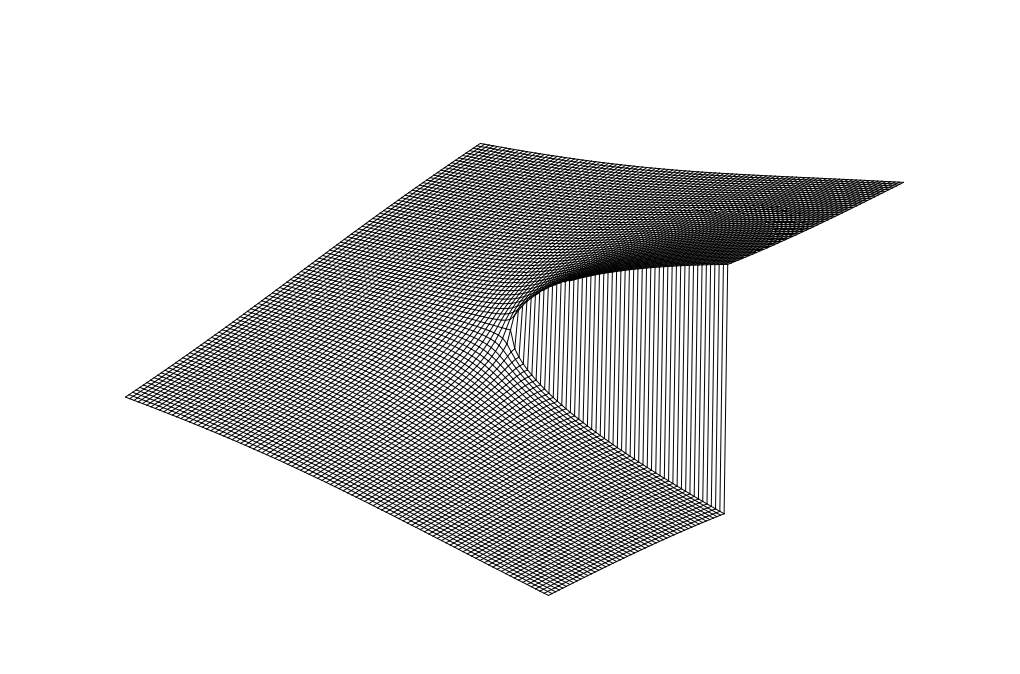
\includegraphics[width=1\linewidth]{sqrprobl}
  \end{minipage} \hfill
  \begin{minipage}{0.49\linewidth}
    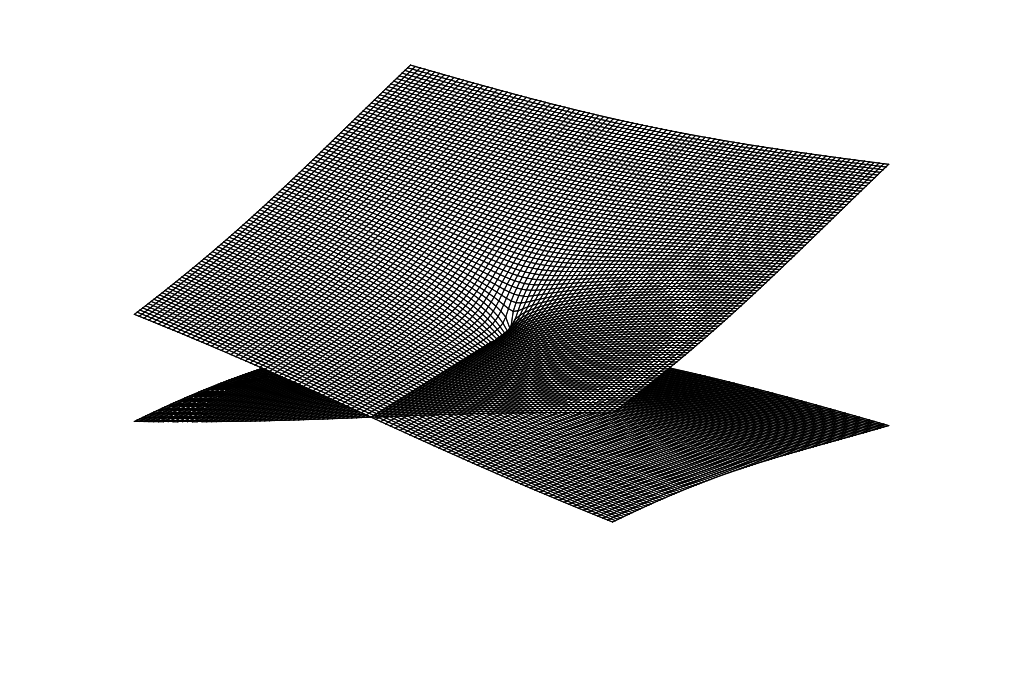
\includegraphics[width=1\linewidth]{sqrootrim}
  \end{minipage}
  \caption{Разрыв мнимой части у корня и риманова поверхность для него}
  \label{fig:sqrtrimsurf}
\end{figure}

\begin{figure}[h]
  \centering
  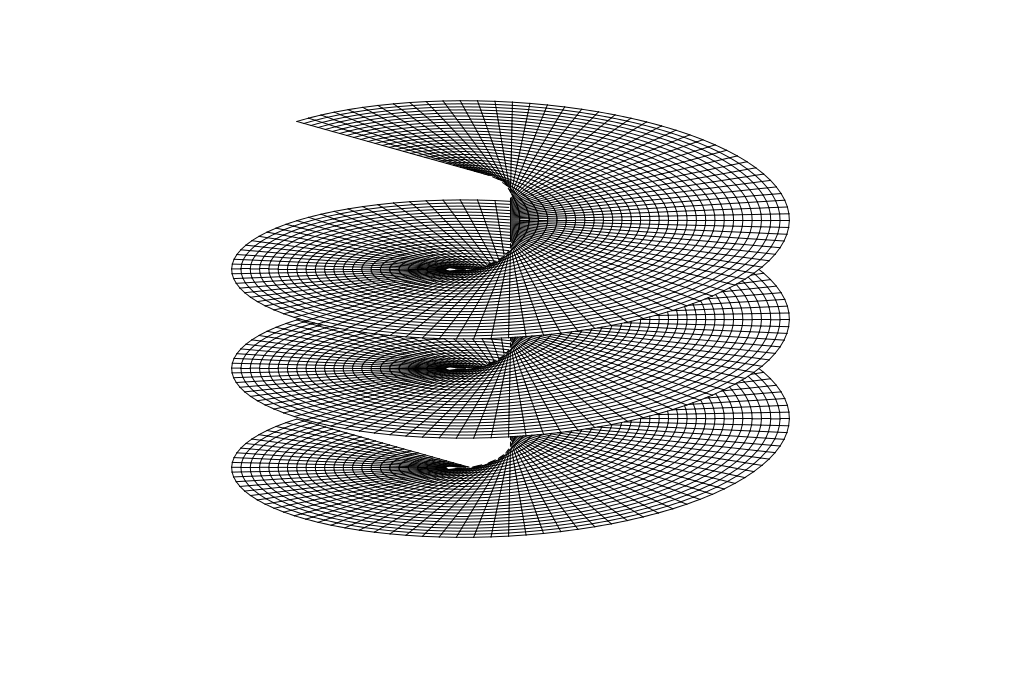
\includegraphics[width=0.8\linewidth]{logrimsurf}
  \caption{Риманова поверхность для логарифма}
  \label{fig:logrimsurf}
\end{figure}




























% <+endofspell+> 
\end{document}
